
\subsection{Transmon qubits}

A Cooper pair box can already work as a qubit, but the its property are not ideal.
In general, we use a variation called \textit{transmon}.\\
A transmon qubit is a CPB shunted by a capacitor that is large in respect to the capacity of the junction.
The result is the characteristic ratio $E_j/E_C \gg 1$ (CPB usually have $E_J/E_C < 1$).

The physical implementation of a transmon is usually very different from a CPB (in particular for XMONs, the main transmon architecture), but the Hamiltonian is always of the same form.
The eigenvalues, however, are extremely dependent on the $E_J/E_C$ ratio, as visible in \cref{fig:levels-ratio}.
\begin{figure}[ht]
    \centering
    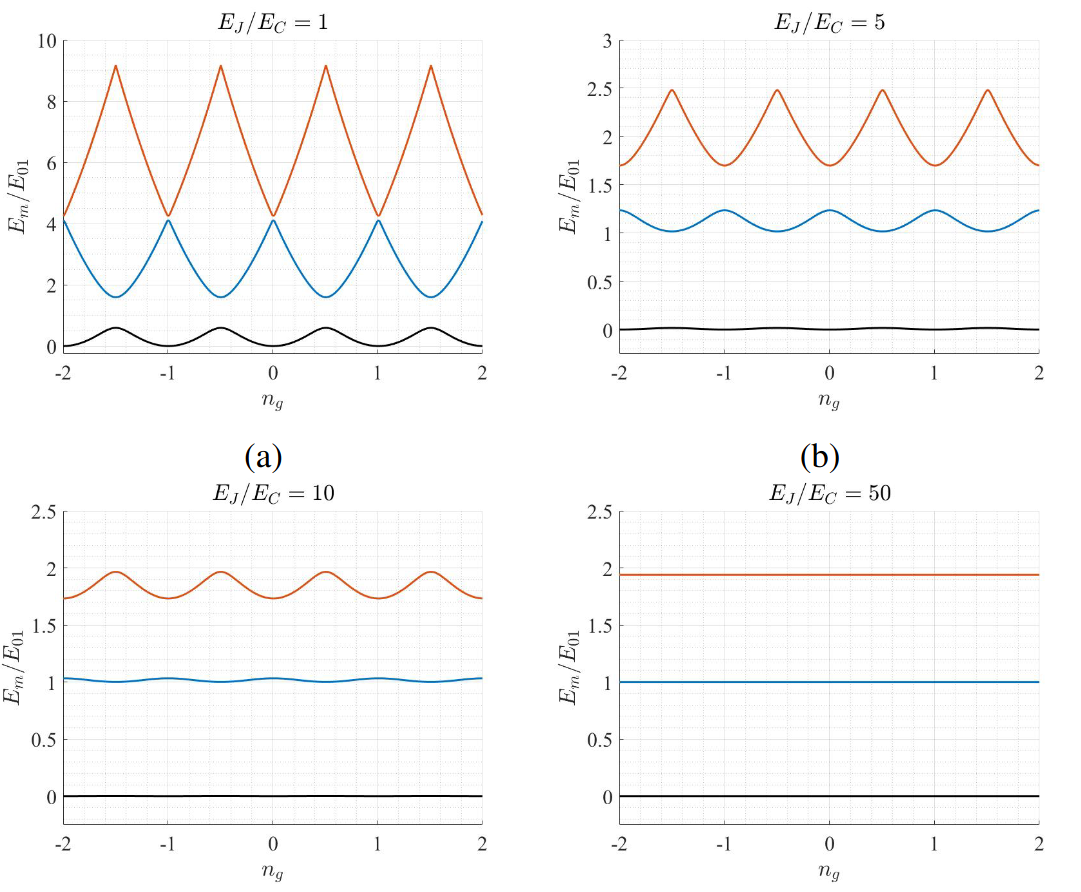
\includegraphics[width=\textwidth]{Theory/figures/levels_ratio.png}
    \caption[Comparison of qubit Hamiltonian eigenvalues for different ratios of $E_J/E_C$.]{Comparison of the Hamiltonian eigenvalues for different ratios of $E_J/E_C$. Credits \cite{Roth2021}.}
    \label{fig:levels-ratio}
\end{figure}
In the transmon limit the energy levels are extremely flat in respect to $n_g$, so much more stable, but also more harmonic.
Since the sensitivity from charge noise decreases faster than the anharmonicity, then we achieve a practical insensitivity from charge noise, while still having enough anharmonicity to consider the system a qubit (typically we have transition of $\approx 10$ GHz and anharmonicities of $\approx 200$ MHz).

The Hamiltonian of this system, derivable from classical circuits Hamiltonians, can be written as:
\begin{equation}\label{eq:hamiltonian_transmon}
    \hat H = 4 E_c (\hat n - n_g ) ^ 2 - E_J \cos \hat\phi
\end{equation}

\subsubsection{Flux tunable qubits}\label{sec:flux_tunable_qubits}

The introduction of a SQUID instead of a single junction leads, as we have seen in \cref{sec:flux_tunable_junction}, to flux tunability of $E_J$. For identical junctions in the SQUID we have:
\begin{equation}
    E_J = E_{j,max} \left|  \cos (\pi \Phi / \Phi_0)  \right|
\end{equation}
where the external magnetic flux is $\Phi$.

This flux dependency will be exploited in two-qubit gates applications, but also has some major drawbacks.

The idea is that, changing $E_J$, the first effect is to change the transition frequency 0-1 of the qubit. This follows the relation:
\begin{equation}
    f (\Phi) \approx \frac{1}{h} \left ( \sqrt{8 E_J E_C \left| \cos \left ( \pi \frac{\Phi}{\Phi_0} \right) \right|} - E_C \right)
\end{equation}

This gets translated into saying that the frequency is tunable by applying external flux, but also that spurious magnetic currents will affect the qubit.

It is currently not possible to completely remove magnetic fluxes "trapped" in a cryostat and the problem becomes worse when you know that, for every warm up the trapped flux changes and the qubit needs to be re-calibrated.

However, flux-tunable qubits offers a straightforward way of implementing two-qubit interactions, "moving" one qubit frequency to the same value of a neighbor qubit, causing hybridization of states and creation of polarons.

Note that the flux-tunable technology is not the only one for implementing two-qubit interactions. For example, IBM, one of the most important player in the superconducting qubit development, never used flux tunable qubits for their backend and even Nakamura's lab (one of the most prominent labs in the word) is moving away from them, because of the problems related to flux-noise.

In any case, it is possible to minimize the sensitivity of the transition frequency, using a special bias value. The charge-degeneracy point $n_g = 1/2$, that identifies the so-called \textit{sweetspot}.
The idea is to move the qubit to its maximum frequency, where we have that higher \textit{and} lower biases both lead to a decrease.

Since the charge dispersion has no slope there, linear noise contributions cannot change the qubit transition frequency.
With this procedure, the unfavorable sensitivity of CPBs to charge noise can be improved significantly, potentially raising T2 times from the nanosecond to the microsecond range.
Unfortunately, the long-time stability of CPBs at the sweet spot still suffers from large fluctuations which drive the system out of the sweet spot and necessitate a resetting of the gate voltage.


